\documentclass[12pt]{article}

%% Escrevendo em português:
\usepackage[brazil]{babel}
\usepackage[latin1]{inputenc} 
\usepackage[T1]{fontenc}
\usepackage{psfrag}
\usepackage{fullpage}
\usepackage{setspace}
\usepackage{graphicx}
\usepackage{epsfig}
\usepackage{epstopdf}
\usepackage{color}
\usepackage{caption}
\usepackage{subcaption}
\usepackage[section]{placeins}
\usepackage{float}
\usepackage{amsmath}

%%%%%%%%%%%%%%%%
\begin{document}
%%%%%%%%%%%%%%%%

\begin{titlepage}

\newcommand{\HRule}{\rule{\linewidth}{0.5mm}} % Defines a new command for the horizontal lines, change thickness here

\center % Center everything on the page
 
%----------------------------------------------------------------------------------------
%	HEADING SECTIONS
%----------------------------------------------------------------------------------------

\textsc{\LARGE Universidade Estadual de Campinas}\\[0.5cm]
\textsc{\normalsize ES827A - Rob�tica Industrial}\\[0.2cm] % Major heading such as course name
\textsc{\normalsize Turma A}\\[0.2cm] % Minor heading such as course title

%----------------------------------------------------------------------------------------
%	TITLE SECTION
%----------------------------------------------------------------------------------------
\vspace {5cm}
{ \huge \bfseries Projeto Final - Din�mica e cinem�tica do rob� Puma560 }\\[0.4cm] % Title of your document
 
%----------------------------------------------------------------------------------------
%	AUTHOR SECTION
%----------------------------------------------------------------------------------------
\vspace {5cm}
\begin{minipage}{0.4\textwidth}
\begin{flushleft} \large
\emph{Alunos:}\\
 \begin{tabbing}
 Augusto Miranda Garcia\hspace{1cm} \=  \= 104627 \\
 Guilherme de Oliveira Souza  \> 117093 \\
 \end{tabbing}
\end{flushleft}
\end{minipage}
\vspace {2cm}

\begin{minipage}{0.4\textwidth}
\begin{flushright} \large
\emph{Professor respons�vel:} \\
Dr. Ely Carneiro Paiva
\end{flushright}
\end{minipage}\\[2cm]

{\large \today}\\[3cm] % Date, change the \today to a set date if you want to be precise

\vfill % Fill the rest of the page with whitespace

\end{titlepage}



\tableofcontents
\clearpage

\section{Objetivo}
\begin{par}
	O objetivo desse relat�rio � apresentar o desenvolvimento dos conceitos apresentados em aula de rob�tica industrial nas atividades propostas para o projeto, sendo ent�o conclu�do com quest�es sobre o assunto desenvolvido. � utilizado para tal o Robotics Toolbox, sendo usado o rob� Puma560, j� inclu�do na toolbox.
\end{par}

\begin{figure}[H]
\centering
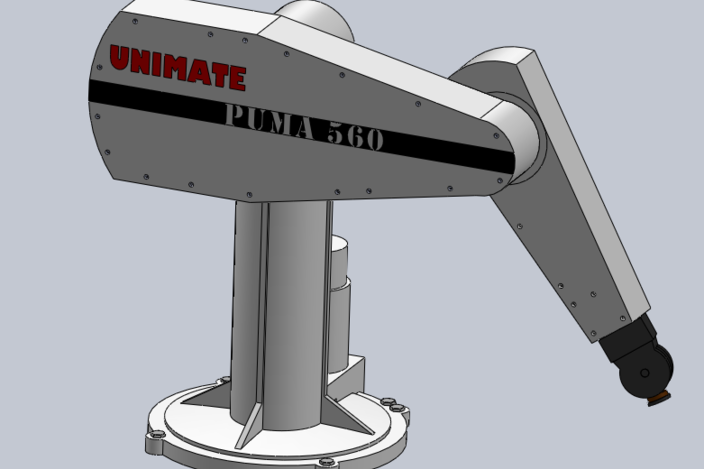
\includegraphics [width=4in]{puma560.png}
\caption {Rob� Puma560.}
\end{figure}

\section{Din�mica}
\begin{par}
	Para a modelagem din�mica do rob� seguiu-se o cap�tulo 6 da tese fornecida no roteiro do projeto, com a ressalva de ter-se evitado o uso do simulink, sendo ao inv�s feita a chamada do rob� e montagem do sistema diretamente em c�digo, que pode ser encontrado nos anexos. Ap�s a montagem, foram feitos testes em malha aberta e an�lise do equil�brio de energia cin�tica do rob�.
\end{par}

\subsection{Simula��es em malha aberta}
\end{document}